\documentclass[11pt]{article}
 
\usepackage[top=0.75in, bottom=1.25in, left=1in, right=1in]{geometry} 
\usepackage{amsmath,amsthm,amssymb} %this is THE math package
\usepackage{mathtools}
\usepackage{tikz}
\usepackage{graphicx}
\usepackage{fancybox}
\usepackage{hyperref}
\usepackage{varwidth}
\usepackage{mdframed}
\usepackage{mathrsfs}
\usepackage[most]{tcolorbox}
%------------------------
%Fonts I use, uncomment if you like to use them.
%The first is the general font, and the second a math font
\usepackage{mathpazo}
\usepackage{eulervm}
\usepackage{graphicx}
\graphicspath{ {./images/} }
%------------------------
%This is so that we have standard fonts for the double-stroked symbols
%for reals, naturals etc. regardless of what font you use.
%Don't comment
\AtBeginDocument{
  \DeclareSymbolFont{AMSb}{U}{msb}{m}{n}
  \DeclareSymbolFontAlphabet{\mathbb}{AMSb}}
%------------------------

%----------------------------------------------
%User-defined environments
%Commented because we're not using them in this document
%The only uncommented ones are the Problem and Solution environment

% \newenvironment{theorem}[2][Theorem]{\begin{trivlist}
% \item[\hskip \labelsep {\bfseries #1}\hskip \labelsep {\bfseries #2.}]}{\end{trivlist}}
% \newenvironment{lemma}[2][Lemma]{\begin{trivlist}
% \item[\hskip \labelsep {\bfseries #1}\hskip \labelsep {\bfseries #2.}]}{\end{trivlist}}
% \newenvironment{exercise}[2][Exercise]{\begin{trivlist}
% \item[\hskip \labelsep {\bfseries #1}\hskip \labelsep {\bfseries #2.}]}{\end{trivlist}}
% \newenvironment{question}[2][Question]{\begin{trivlist}
% \item[\hskip \labelsep {\bfseries #1}\hskip \labelsep {\bfseries #2.}]}{\end{trivlist}}
% \newenvironment{corollary}[2][Corollary]{\begin{trivlist}
% \item[\hskip \labelsep {\bfseries #1}\hskip \labelsep {\bfseries #2.}]}{\end{trivlist}}
\newenvironment{problem}[2][Problem\!]{\begin{trivlist}
\item[\hskip \labelsep {\bfseries #1}\hskip \labelsep {\bfseries #2}]}{\end{trivlist}}
%\newenvironment{sub-problem}[2][]{\begin{trivlist}
%\item[\hskip \labelsep {\bfseries #1}\hskip \labelsep {\bfseries #2}]}{\end{trivlist}}
\newenvironment{solution}{\begin{proof}[\textbf{\textit{Solution}}] }{\end{proof}}
%----------------------------------------------

%----------------------------
%User-defined notations
\newcommand{\zz}{\mathbb Z}   %blackboard bold Z
\newcommand{\qq}{\mathbb Q}   %blackboard bold Q
\newcommand{\ff}{\mathbb F}   %blackboard bold F
\newcommand{\rr}{\mathbb R}   %blackboard bold R
\newcommand{\nn}{\mathbb N}   %blackboard bold N
\newcommand{\cc}{\mathbb C}   %blackboard bold C
\newcommand{\af}{\mathbb A}   %blackboard bold A
\newcommand{\pp}{\mathbb P}   %blackboard bold P
\newcommand{\id}{\operatorname{id}} %for identity map
\newcommand{\im}{\operatorname{im}} %for image of a function
\newcommand{\dom}{\operatorname{dom}} %for domain of a function
\newcommand{\cat}[1]{\mathscr{#1}}   %calligraphic category
\newcommand{\abs}[1]{\left\lvert#1\right\rvert} %for absolute value
\newcommand{\norm}[1]{\left\lVert#1\right\rVert} %for norm
\newcommand{\modar}[1]{\text{ mod }{#1}} %for modular arithmetic
\newcommand{\set}[1]{\left\{#1\right\}} %for set
\newcommand{\setp}[2]{\left\{#1\ \middle|\ #2\right\}} %for set with a property
\newcommand{\card}[1]{\#\,{#1}} %for cardinality of a set
\newcommand\m[1]{\begin{pmatrix}#1\end{pmatrix}} 

%Re-defined notations
\renewcommand{\epsilon}{\varepsilon}
\renewcommand{\phi}{\varphi}
\renewcommand{\emptyset}{\varnothing}
\renewcommand{\geq}{\geqslant}
\renewcommand{\leq}{\leqslant}
\renewcommand{\Re}{\operatorname{Re}}
\renewcommand{\Im}{\operatorname{Im}}
%----------------------------

\allowdisplaybreaks
 
 
\begin{document}
 
\title{Assignment}
\author{Kevin Guillen\\[0.5em]
MATH  | Class | Quarter}
\date{} 
\maketitle
\newpage

\tableofcontents
\newpage
%Use \[...\] instead of $$...$$
\section{$C^{3}$ Solutions Submitted for Portfolio}
\subsection{I.C. Solutions}
\begin{itemize}
    \item[\text{Oct 4 Sub. }]  \begin{itemize}
        \item[14] Get your hands dirty
        \item[19] Recurrence relations
    \end{itemize}
    \item[\text{Nov 1 Sub. }] \begin{itemize}
        \item[81] Arithmetic and Geometric sequences and series
        \item[99] Inequalities, factor tactic
    \end{itemize}
    \item[\text{Nov 8 Sub. }]  \begin{itemize}
        \item[122] Specialization, Intermediate Goals, Getting your hands dirty
        \item[110] Intermediate goals, Getting your hands dirty, Counting in two ways
    \end{itemize}
    \item[\text{Nov 15 Sub. }] \begin{itemize}
        \item[143] Primes and divisibility, congruence, Penultimate step
    \end{itemize}
    \item[\text{Nov 19 ReSub. }] \begin{itemize}
        \item[135] Primes and divisibility, congruence, factor tactic
        \item[136] Primes and div, congruence
    \end{itemize}
    \item[\text{Nov 22 Sub. }] \begin{itemize}
        \item[148] Putnam - Geometry, Wishful thinking
        \item[153] Geometry, Penultimate step
    \end{itemize}
    \item[\text{Dec 3 ReSub. }]\begin{itemize}
        \item[46] Get your hands dirty, Penultimate step
        \item[109] Generating functions
    \end{itemize}

\end{itemize}

\subsection{O.C. Solutions}
\begin{itemize}
    \item[\text{Sept 27 Sub. }] \begin{itemize}
        \item[1] Arithmetic and Geometric sequences and series, Binomial Expansion
    \end{itemize}
    \item[\text{Oct 4 Sub. }] \begin{itemize}
        \item[18] Getting your hands dirty, Relax Conditions
    \end{itemize}
    \item[\text{Nov 8 Sub. }] \begin{itemize}
        \item[69] Wishful thinking, Partitions and Bijections
        \item[71] Get your hands dirty
    \end{itemize}
    \item[\text{Nov 15 Sub. }] \begin{itemize}
        \item[90] Get your hands dirty, Factor tactic 
    \end{itemize}
    \item[\text{Nov 22 Sub. }] \begin{itemize}
        \item[72] Get your hands dirty
        \item[77] Get your hands dirty
        \item[83] Recurrence relations, Primes and divisibility
    \end{itemize}
    \item[\text{Dec 3 ReSub.}]\begin{itemize}
        \item[68] Relax Conditions, Specialization, Graph Theory 
    \end{itemize}
\end{itemize}

\subsection{Putnam Solutions}
\begin{itemize}
    \item[\text{Nov 29 Sub. }]\begin{itemize}
        \item[PP14] Specialization, Polynomials
        \item[PP15] Wishful thinking, Find and exploit symmetries
    \end{itemize}
    \item[\text{Dec 6 Sub. }]\begin{itemize}
        \item[PP19] Get your hands dirty, congruence, Factor Tactic
        \item[PP20] Get your hands dirty, Wishful thinking, Penultimate step
        \item[PP29] Congruence, Inequalities, Arithmetic and geometric sequences and series, Get your hands dirty, Factor tactic 
        \item[PP37]  Penultimate, Factor Tactic 
        \item[PP40] Find and exploits symmetries, Geometry
        \item[PP41] Factor tactic, Get your hands dirty, Wishful thinking
        \item[PP42] Diophantine equation, Factor tactic, Primes and divisibility 
    \end{itemize}
\end{itemize}

\subsection{I.C. Solutions being Resubmitted} 
\begin{itemize}
    \item[\text{Dec 3 ReSub. }]\begin{itemize}
        \item[44] Invariance Principle
    \item[50] Graph Theory
    \item[151] Geometry
    \end{itemize}
\end{itemize}
\subsection{O.C. Solutions being Resubmitted}
\begin{itemize}
    \item[\text{Dec 3 ReSub.}] \begin{itemize}
        \item[30] Pigeon Hole Principle
    \end{itemize}
\end{itemize}

\subsection{New I.C. Submissions}
\begin{itemize}
    \item[124] Partitions and Bijections, Wishful thinking
\end{itemize}

\section{Resubmissions}
\begin{tcolorbox}
    \begin{problem}{10/11 IC (44.)} 
        The numbers $1,2,\dots, 50$ are written on the blackboard. Then two numbers $a$ and $b$ are chosen and replaced by the single number $\abs{a-b}$. After 49 operations a single number is left. Prove that it is odd. 
    \end{problem}
\end{tcolorbox}

\begin{proof}
    If we have the numbers $1,2,\dots, 50$ that means half of them are even and half are odd. In other words we have 25 even numbers and 25 odd numbers. We know after 49 operations we will have a single number left. To determine if it is odd or even let's look at the 3 scenarios when taking the differences of even and odd numbers.
    \begin{alignat*}{2}
        &\text{Two even numbers: } 2k - 2l &&= 2(k-l) \\
        &\text{Odd and even numbers: } 2k + 1 - 2l &&= 2(k-l) + 1 \\
        &\text{Two odd numbers: } 2k + 1 - (2l + 1) &&= 2(k-l)
    \end{alignat*}

    Therefore the number of odd numbers removed by using any operation will be either 0 or 2, meaning the parity of the number of odd numbers is invariant
\end{proof}
\newpage
\begin{tcolorbox}
    \begin{problem}{10/13 IC (50.)} 
        Every room in a house has an even number of doors. Prove that there are an even number of entrance doors to the house. 
    \end{problem}
\end{tcolorbox}
\begin{solution}
    Let each room in the house be a vertex and outside be a vertex as well. All we have to show now is that this graph can't have exactly one vertex of odd degree. By the handshaking lemma there does not exist any such graph. Meaning the vertex corresponding to the outside is also even. 
\end{solution}

\begin{tcolorbox}
    \begin{problem} {IC | 11/15 | 151.}
        Is it possible for a triangle to have altitudes equal to 6, 10, and 20?
    \end{problem}
\end{tcolorbox}
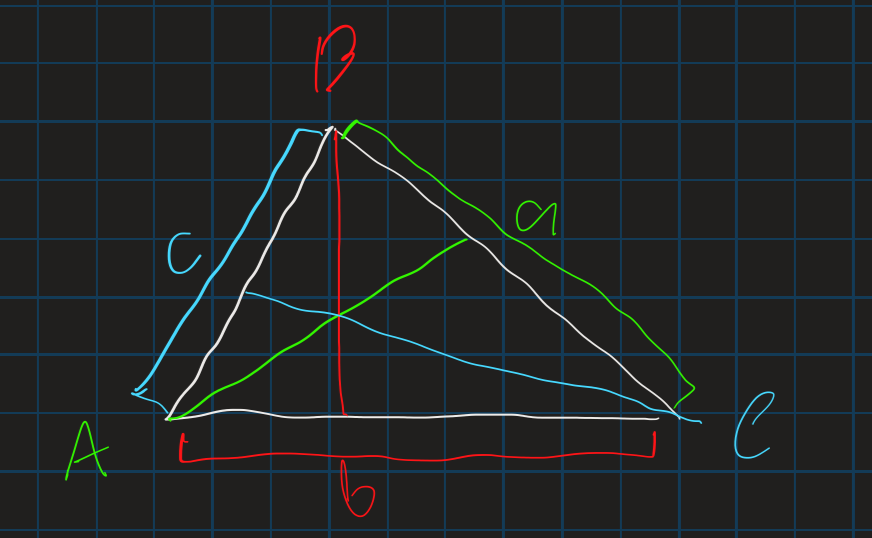
\includegraphics[scale=.5]{prob2}
\begin{proof}
    Consider the area of the triangle drawn above. It will be the following,
    \[A = \frac{6}{2}a = \frac{10}{2}b = \frac{20}{2}c.\]

    Which gives us the following equations,
    \begin{align*}
        a &= \frac{1}{3}A \\
        b &= \frac{1}{5}A \\
        c &= \frac{1}{10}A
    \end{align*}

    Recall though the sum of any 2 sides of a triangle has to be greater than the remaining third side. Which means we must have (triangle inequality)
    \begin{align*}
        a &< b + c \\
        \frac{10}{30}A &< \frac{6}{30}A + \frac{3}{10}A = \frac{9}{10}A
    \end{align*}
    that is if our altitudes were 6, 10 and 20, that would imply $\dfrac{10}{30}A < \dfrac{9}{10}A$ which is a contradiction. Therefore there can not be a triangle with those given altitudes. 
\end{proof}

\newpage
\begin{tcolorbox}
    \begin{problem}{10/8 | OC | 30. }
        Chose any $(n+1)$ element subset of $\set{1,2,\dots, 2n}$. Show that this subset contains two elements which are relatively prime. 
    \end{problem}
\end{tcolorbox}
\begin{proof}
    Let $S$ denote the set $\set{1,2,\dots,2n}$. To prove this we will use the pigeon hole principle and the fact that two neighboring numbers are relatively prime. Our "pigeonholes" in this case will be a list of $n$ numbers from $S$ in ascending order where every number is not adjacent to any other number.  The max amount of numbers that can be chosen from $\set{1,2, \dots , 2n}$ such that no numbers are relatively prime would be $n$, because consecutive numbers in our list will have a difference of at least 2. So if we choose $n+1$ numbers and match them with our pigeonholes we won't be able to give each number its own hole because there is only $n$ numbers in $S$ that can be not adjacent to any other number, meaning 1 number has to be adjacent to some other number making them relatively prime. 
\end{proof}

\section{New Submissions}
\begin{tcolorbox}
    \begin{problem}{ IC | 11/05 | 124. (Putnam)}
        Define a selfish set to be a set which has its own cardinality as an element. FInd, with a proof, the number of subsets of $\set{1,2,\dots, n}$ which are minimal selfish sets, that is, selfish sets none of whose proper subsets is selfish. 
    \end{problem}
\end{tcolorbox}
\begin{proof}
    Consider an arbitrary set $A$. If $A$ were to be a minimal selfish set, then by definition every element of $A$ would need to be greater than or equal to the cardinality of $A$. This observation will be needed. 

    Let $A_n$ be defined as follows,
    \[A_n := \set{1,2,\dots, n}.\]
    Also let $S(A_n)$ denote the number of subsets where are minimal selfish sets in $A_n$.


    Let $B \subseteq A$ and be a minimal selfish set. There are 2 cases here, the first is that $n$ is in $B$ and the second is that $n$ is not in $B$.
    
    If $n$ is not contained in $B$ then we know know $B$ will also have to be a minimal selfish set of $A_{n-1}$ which there are $S(A_{n-1})$ of. 

    If $n$ is indeed contained in $B$ then we know that the element 1 cannot be in $B$ because then $B$ would not be a minimal selfish set. This is because $\set{1}$ is a minimal selfish set. So this subset must also be a subset of $\set{2, \dots, n}$. If we remove the element $n$ from this set then we know it must be a subset of $\set{2, \dots, n-1}$. Next if we were to subtract 1 from every element this new set, let's refer to it as $C$, has got to be a subset of $\set{1,\dots,n-2}$. Meaning if $B$ was a minimal selfish set of $A_n$ that contained $n$, then our derived set $C$, must be a minimal selfish set of $A_{n-2}$. Which we know there are $S(A_{n-2})$ of. 
    
    Putting this together we get,
    \[S(A_n) = S(A_{n-1} + S(A_{n-2})).\]

    We see for $A_1 = \set{1}$. That it only has 1 subset that is a minimal selfish set, that it $\set{1}$. Next we see for $A_2 = \set{1,2}$ that it only contains 1 subset that is a minimal selfish set at that is $\set{1}$ again. So we have $A_1 = A_2 = 1$. Notice though that these are the same starting values as the fibonacci sequence, and that we define the value of $S(A_n)$ for $n > 2$ as the sum of the previous 2 terms. Thus $S(A_n) = \text{Fib}(n)$, where $\text{Fib}(n)$ is the $n$th term in the fibonacci sequence. 
\end{proof}

\newpage
\section{Strategies}
\begin{description}
    \item[Generalization]
    \item[Specialization] IC 122, OC 68, PP14
    \item[Relax conditions] OC 18, 68
    \item[Get your hands dirty] IC: 14, 46 OC: 71, 72, 77, 90 Putnam: 19, 20, 41
    \item[Wishful thinking] IC: 148 OC: 69 Putnam: 15, 20, 41 
    \item[Find a penultimate step] IC: 143, 153, 46 Putnam: 20, 37
    \item[Formulate intermediate goals] IC: 122, 110     
\end{description}

\section{Tactics and techniques}
\begin{description}
    \item[External principle]
    \item[Find and exploit symmetries] Putnam: 15
    \item[Invariance principle] IC: 44
    \item[Pigeon hole principle] OC: 30
    \item[Counting in two different ways] IC 110
\end{description}


\section{Tools and mathematical content}
\begin{description}
    \item[Graph Theory] IC: 50 OC: 68
    \item[Complex numbers]
    \item[Generating functions] IC: 109
    \item[Factor tactic]IC: 99, 135 OC: 90 Putnam: 19, 29,37, 41, 412 
    \item[Arithmetic and geometric sequences and series] IC: 81, OC sept 27 Putnam: 29
    \item[Polynomials] Putnam: 14
    \item[Inequalities] IC:99 Putnam: 29
    \item[Pascal's triangle and the binomial theorem] OC: 1
    \item[Partitions and bijections] OC: 69
    \item[Principle of inclusions-exclusion]
    \item[Recurrence relations] IC: 19, OC: 83
    \item[Primes and divisibility] IC: 143, 135, 136 OC: 83 Putnam: 42
    \item[Congruence] IC: 143, 135, 136 Putnam: 19, 29
    \item[Diophantine equations] Putnam: 42
    \item[Geometry] IC 148, 151, 153 Putnam: 40         
\end{description}



\end{document}